Different methods of software development exist in software engineering. A different type of development means a different way of testing, so it is important to choose a proper development process before a team starts developing. This chapter explains the development methods and how to organise performance regression testing when using each of these methods.

\section{Code-and-fix model}
``The basic model used during the early days of software devolpment contained two steps: write some code and fix the problems in the code'' \cite{boehm1988spiral} This `method' is not appropriate for performance regression testing, because of the poor preparation of testing. It is hard to write test suites without a plan and knowledge of the overall design.

\section{Waterfall method}
``The waterfall method establishes a sequence of stages-requirements, specifications, design, coding, testing and maintenance-to guide the development process. ''\cite{kang1989software}. The sequences of the waterfall method will be done until the development of the system is completed. The waterfall method even became the basis for most software acquisition standards in the past years. \cite{boehm1988spiral}. This type of developing has a testing phase. Collins et al studied an agile waterfall process. \cite{collins2010iterative} A figure giving the phases of the waterfall development process are shown below.

\begin{figure}[H]
\begin{center}
  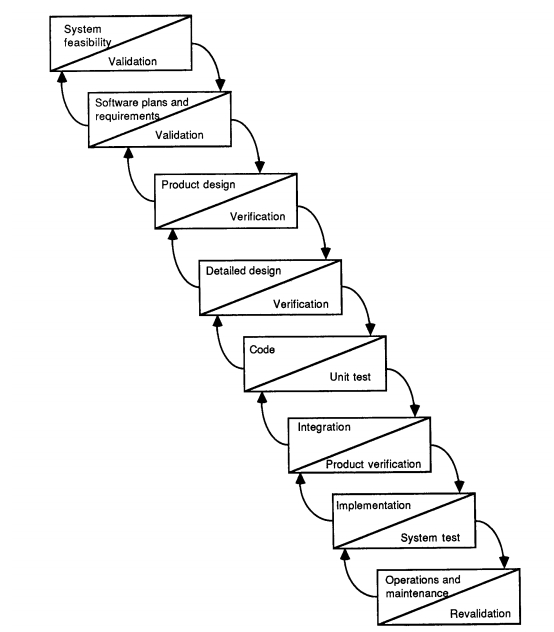
\includegraphics[width=0.5\textwidth]{Figures/waterfall.jpg}
\end{center}
  \caption{Phases during a waterfall development process\cite{boehm1988spiral}} 
\end{figure}

Each rectangle in the figure states as a phase in the waterfall development process. When something goes wrong during the process it will be checked if the errors occurred in the current states. If not, the previous state will be checked. The waterfall method is a static development process. The waterfall method is a static development process. The testing is done near the end of the process, which means that performance regressions are tested near the end of the process too. This suggests that performance regression testing will not be effective, because the tests will be runned when the implementation (almost) done. Although, when using an iterative form of the waterfall method, it can be tested effective. A research showed that, when using an iterative process, regression testing using the waterfall method can be very useful. It even has been stated that most of the time performance is the biggest issue in the field. \cite{foo2010mining} The combination of performance as biggest issue and an effective way of regression testing when using an iterative waterfall process suggests that performance regression testing can be done effective here too.

\section{Spiral method}
``The spiral method creates a risk-driven approach to the software process rather than a primarily document-driven or code-driven process. It incorporates many of the strengths
of other models and resolves many of their
difficulties.''\cite{boehm1988spiral} The phases of the spiral development process are shown in the figure below. 

\begin{figure}[H]
\begin{center}
  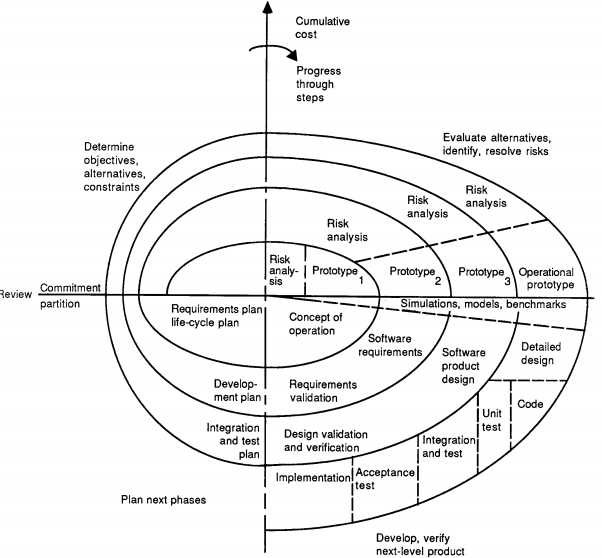
\includegraphics[width=0.5\textwidth]{Figures/spiral.jpg}
\end{center}
  \caption{Phases during a spiral development process\cite{boehm1988spiral}} 
\end{figure}

When using the spiral model, the main focus lies on the different risks of a software project. Examples of these risks are: low budget, developing wrong functions or a continous change of functions. These development processes are divided by the property of their risks. Different prototypes will be made implementing the risks. Performance regression testing can be seen as a risk too, because you have to maintain the performance when a later prototype is made. This means that the spiral method can be effective when using the spiral method.

\section{Scrum}
``Scrum is an Agile software development process designed to add energy, focus, clarity, and transparency to project teams developing software systems.''\cite{sutherland2007distributed} A Scrum development process is divided into three kinds of phases. Research has been done to show that automated regression tests during the daily builds will greatly improve the quality of the product \cite{Future_of_Scrum}. This means that Scrum is a useful development method for regression testing. When the performance is monitored here as well, it  \\ There are two organising phases, which are the opening and closing phases and the last phase is the sprint phase which is further divided. The planning and closing phases are organising phases. It is not necessary to run tests here, because there is either no code (opening) or all the performance regression tests have been executed and passed (closing). Though, planning when to test is an example of an organising aspect which can be done during the opening phase and verifying that the test suite covers all the code can be done during the closing phase. \\ The actual creation of tests will be done during the sprints. The sprints consist of developing, wrapping, reviewing and adjusing. The wrapping part of the sprint, combines all the implemented code. This process of wrapping is a very appropriate moment to test for performance regressions. \\

\section{General aspects of test organization}
Despite the fact that the development method is significant, there are some other organising aspects which could make a difference in the way of performance regression testing. \\
First of all, it is important who will do the testing. Zaparanuks et al. performed an experiment in which one person did all the testing throughout the project. \cite{sutherland2009fully} This person is an active member of the team and watches all the members of the developing team. This method provides a way to deal with any issues that could come up during the process. The appointed person will directly try to deal with issues coming up by the members of the developing team. By appointing this person, the quality of the product is watched the whole time during the project, instead of comparison to the other research where performance regression testing is done during the merge phase. This experiment indicated that the quality of the development got a much higher average score compared to other similar development products. So appointing one tester who only has the task to watch over the quality by testing and for our sake performing regression tests, can have an improved effect on the overall process. \\

Another organising aspect is to make sure a proper test suite is written before programming, and that this test suite is maintained during the project. Test suites should be made with some conditions in mind. Writing complete test suites for complex systems will require the regression testing to run for a long time. \cite{rothermel2001prioritizing} So the developers have to decide to either test the complete system, or to write selective test suites. These test suites will only test the main functionality of the system. \\
After deciding the organising aspects, the actual implementation will be initiated. From now on performance regression testing will be done throughout the process. The developers will decide what kind of data of the implementation will be tested. Performance counters can be used to help decide which data the tests will cover.
